\documentclass[12pt, letterpaper, titlepage]{article}
\usepackage[utf8]{inputenc}
\usepackage{geometry}
\usepackage{color,graphicx,overpic} 
\usepackage{fancyhdr}
\usepackage{amsmath,amsthm,amsfonts,amssymb}
\usepackage{mathtools}
\usepackage{hyperref}
\usepackage{multicol}
\usepackage{array}
\usepackage{float}
\usepackage{blindtext}
\usepackage{longtable}
\usepackage{scrextend}
\usepackage[font=small,labelfont=bf]{caption}
\usepackage[framemethod=tikz]{mdframed}
\usepackage{calc}
\usepackage{titlesec}
\usepackage{listings}
\usepackage[normalem]{ulem}
\usepackage{tabularx}
\usepackage{mathrsfs}
\usepackage{bookmark}
\usepackage{setspace}
\usepackage{tabularx}
\usepackage{ltablex}
\usepackage{enumerate}

\mathtoolsset{showonlyrefs}  
\allowdisplaybreaks

\definecolor{mycolor}{rgb}{0, 0, 0}

\geometry{top=2.54cm, left=2.54cm, right=2.54cm, bottom=2.54cm}
\setlength{\headheight}{20pt}
\setlength{\parskip}{0.3cm}
\setlength{\parindent}{1cm}

\pagestyle{fancy}
\fancyhf{}
\rhead{Lora Ma - 1570935}
\lhead{\textit{ECE 322 Assignment 5}}
\rfoot{Page \thepage}

\begin{document} 
\singlespacing
\section*{Q1}
\begin{enumerate}[a)]
    \item Compound decisions are treated \textit{en bloc} \\
    Cyclomatic complexity = 5 \\
    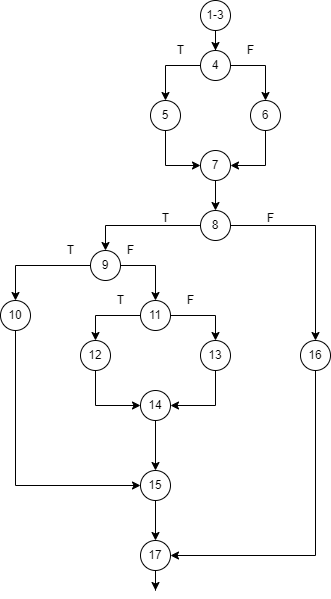
\includegraphics[scale=0.39]{Image1.png}
    \item Compound decisions are treated separately \\
    Cyclomatic complexity = 10 \\
    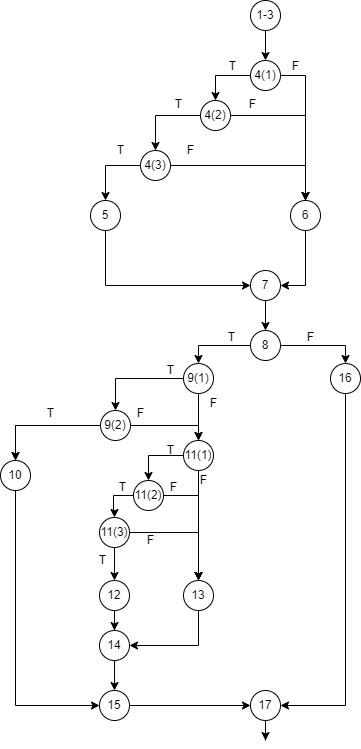
\includegraphics[scale=0.39]{Image2.png}
\end{enumerate}
\section*{Q2}
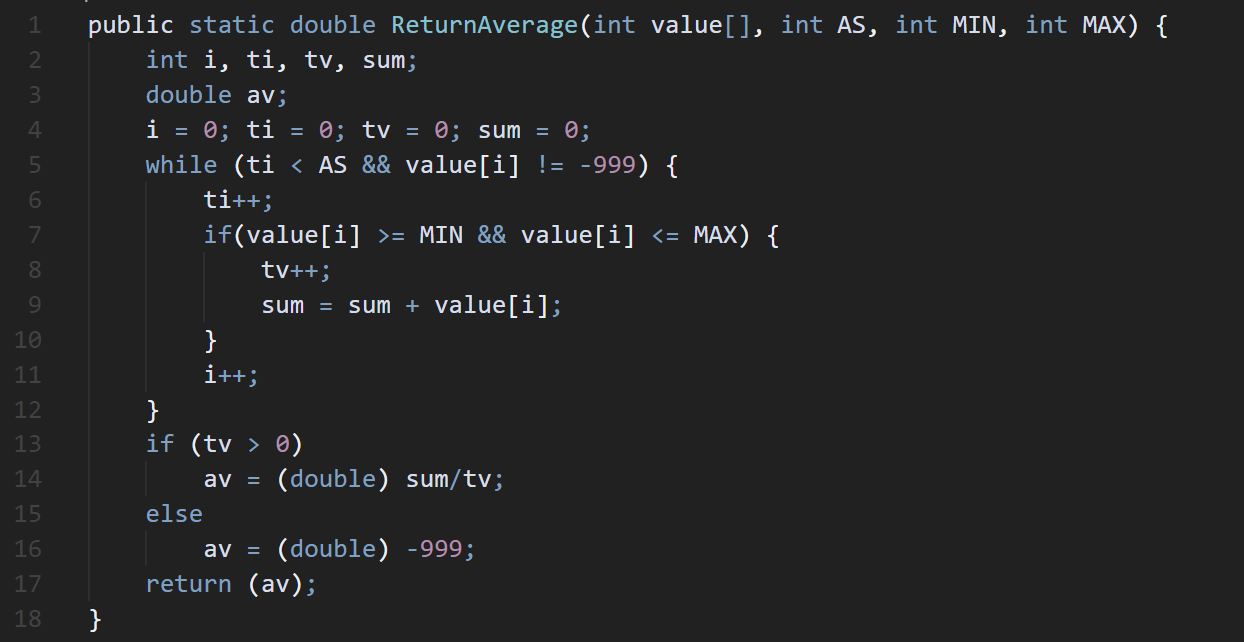
\includegraphics[scale=0.89]{code.png} \\\\
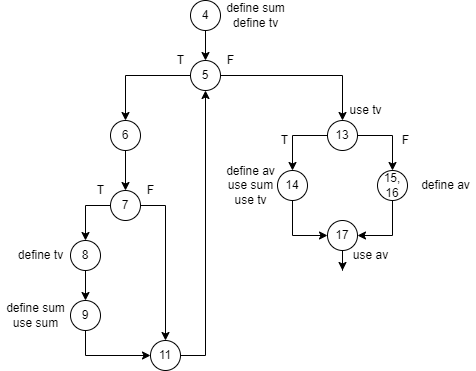
\includegraphics[scale=0.6]{Image3.png} \\
Some \textit{def-clear} paths are as following:\\\\
For tv:
\begin{enumerate}
    \item ($4 \rightarrow  5 \rightarrow 6 \rightarrow 7$)
    \item ($8 \rightarrow 9 \rightarrow 11 \rightarrow 5 \rightarrow 13$)
    \item ($8 \rightarrow 9 \rightarrow 11 \rightarrow 5 \rightarrow 6 \rightarrow 7 \rightarrow 11 \rightarrow 5 \rightarrow 13$)
    \item ($4 \rightarrow  5 \rightarrow 6 \rightarrow 7 \rightarrow 11 \rightarrow 5 \rightarrow 13$)
\end{enumerate}
For av:
\begin{enumerate}
    \item ($14 \rightarrow 17$)
    \item ($16 \rightarrow 17$)
\end{enumerate}
For sum: 
\begin{enumerate}
    \item ($4 \rightarrow 5 \rightarrow 6 \rightarrow 7 \rightarrow 8$)
    \item ($4 \rightarrow 5 \rightarrow 6 \rightarrow 7 \rightarrow 11 \rightarrow 5 \rightarrow 6 \rightarrow 7 \rightarrow 8$)
    \item ($9 \rightarrow 11 \rightarrow 5 \rightarrow 6 \rightarrow 7 \rightarrow 11 \rightarrow 5 \rightarrow 13 \rightarrow 14 $)

\end{enumerate}

\section*{Q3}
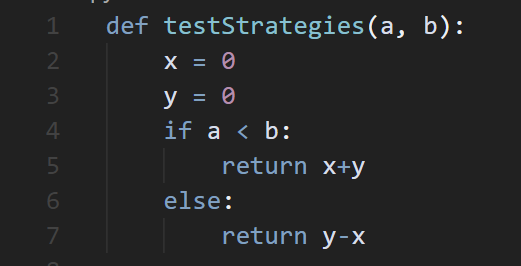
\includegraphics{code1.png}

\section*{Q4}
\begin{table}[H]
    \begin{tabular}{|l|l|l|l|l|l|}
    \hline
    Test \# & a & b & c & d & Expected \\ \hline
    1       & T & F & T & F & T        \\ \hline
    2       & T & F & F & T & T        \\ \hline
    3       & F & F & F & F & F        \\ \hline
    4       & T & T & T & T & F        \\ \hline
    \end{tabular}
    \end{table}

\end{document}  